\documentclass[xcolor=table]{beamer}

\usepackage{amsmath}
\usepackage{amssymb}
\usepackage[utf8]{inputenc}

\usepackage{hyperref}

\usepackage{amssymb} %for Lagrangian L, order O

%\usepackage{gensymb}
\usepackage{siunitx}
\usepackage{xcolor}
\usepackage{colortbl}
\usepackage{cancel}
\usepackage[normalem]{ulem}
\usepackage{calc}
\usepackage{ragged2e}
\usepackage{capt-of}

%for side-by-side figures
\usepackage{graphicx}
\usepackage[compatibility=false]{caption}

\setlength{\parindent}{2em}
\setlength{\parskip}{1em}
\renewcommand{\baselinestretch}{1.1}
\setlength\parindent{0pt} % Removes all indentation from paragraphs - comment this line for an assignment with lots of text

\usetheme{PaloAlto}	%or PaloAlto?
%\usecolortheme{beaver}

\setbeamertemplate{footline}[frame number]

\definecolor{green}{HTML}{C4E76D}
\definecolor{red}{HTML}{F57F73}
\definecolor{yellow}{HTML}{F5E274}

%----------------------------------------------------------------------------------------
%	TITLE SECTION
%----------------------------------------------------------------------------------------
\title[Literature Review: $\tau\to\ell\gamma$ search] %optional
{A search for $\tau\to\ell\gamma$ at Belle}
 
\subtitle{}
 
\author[Braden Moore] % (optional, for multiple authors)
{Braden~Moore}
 
\institute[] % (optional)
{
  School of Physics\\
  The University of Melbourne\\
  \vspace{0.5cm}
  Under the supervision of Dr. Phillip Urquijo
}
 
\date[19 May 2016] % (optional)
 
\logo{
\includegraphics[height=1.5cm]{images/university-of-melbourne-logo.jpg}}

%\setbeamerfont{caption}{size=\footnotesize}


%----------------------------------------------------------------------------------------
\begin{document}
 
\frame{\titlepage}
\fontsize{9pt}{14}\selectfont

%------------------------------

\begin{frame}

\begin{center}
{\Huge Introduction}
\end{center}

\end{frame}

%------------------------------

\begin{frame}
\frametitle{Introduction}

\begin{equation*}
\tau\to\ell\gamma\quad(\ell=\mu,e)
\end{equation*}
\begin{itemize}
\item immeasurably small branching fraction via SM processes
\item lepton flavour violation (LFV) is predictd to appear in a wide variety of New Physics (NP) processes
\item of the $\tau$ processes, decays $\tau\to\ell\gamma$ predicted to be most dominant
\end{itemize}


\end{frame}


%------------------------------

\begin{frame}
\frametitle{Introduction}

\begin{center}
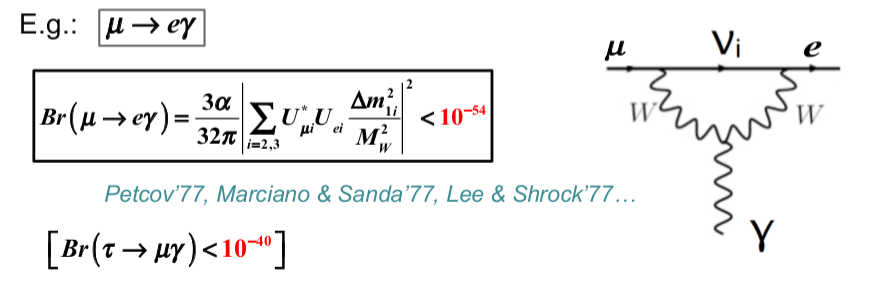
\includegraphics[width=0.8\textwidth]{images/tau-SM-BF.png}
%\caption{$\tau\to\ell\gamma$ branching fractions in SM with massive neutrinos}
\end{center}

\begin{itemize}
\item In the SM with massive neutrinos, the LFV vertices are tiny due to GIM suppression!
\item LFV has unobservably small rates via these processes
\end{itemize}



\end{frame}


%------------------------------



\begin{frame}
\frametitle{Introduction}

\begin{center}
Observation of LFV of this type would be \\an unambiguous signature of NP!
\end{center}

\end{frame}


%------------------------------


\begin{frame}

\begin{center}
{\Huge Obligatory Belle slides}
\end{center}

\end{frame}

%------------------------------


\begin{frame}
\frametitle{Obligatory Belle slides}

\begin{center}
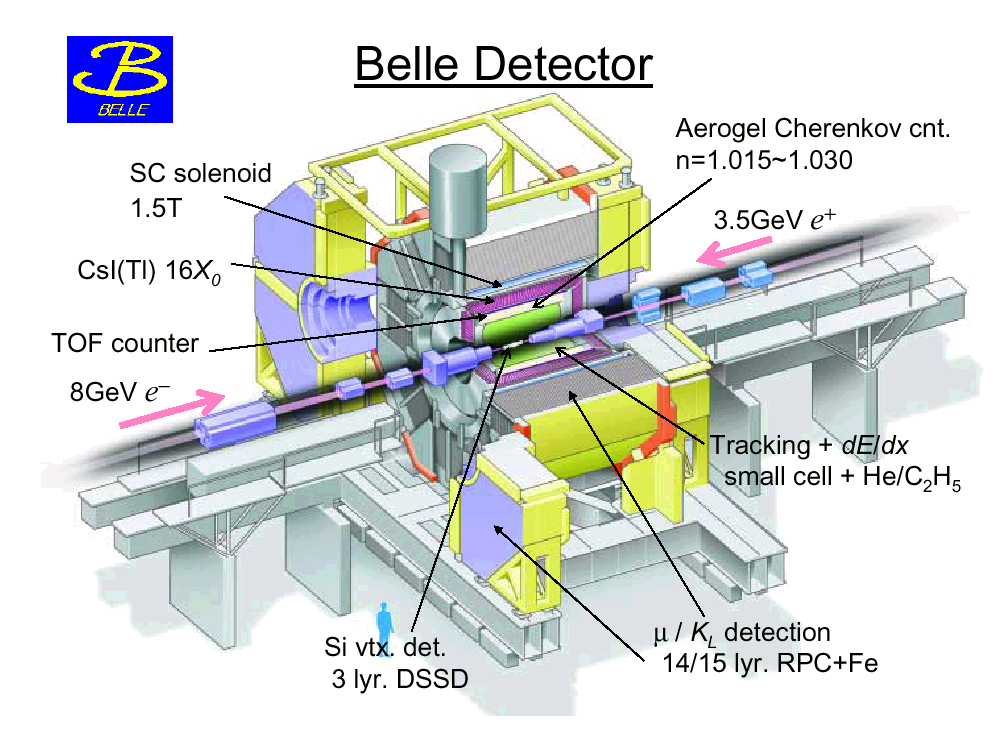
\includegraphics[width=0.8\textwidth]{images/belle-detector.png}
\end{center}

\end{frame}


%------------------------------


\begin{frame}
\frametitle{Obligatory Belle slides}

\begin{itemize}
\item Belle experiment ran from 1998-2011 and collected $\SI{1000}{fb^{-1}}$ of data
\item $e^+ e^-$ asymmetric beam collider ($\SI{8}{GeV}$ and $\SI{3.5}{GeV}$)
\item can produce other tau-pairs via
\begin{equation*}
e^+ e^- \to \tau^+ \tau^-
\end{equation*}
\end{itemize}


\end{frame}




%------------------------------

\begin{frame}

\begin{center}
{\Huge The Standard Model}
\end{center}

\end{frame}

%------------------------------

\begin{frame}
\frametitle{Standard Model (SM)}

\begin{center}
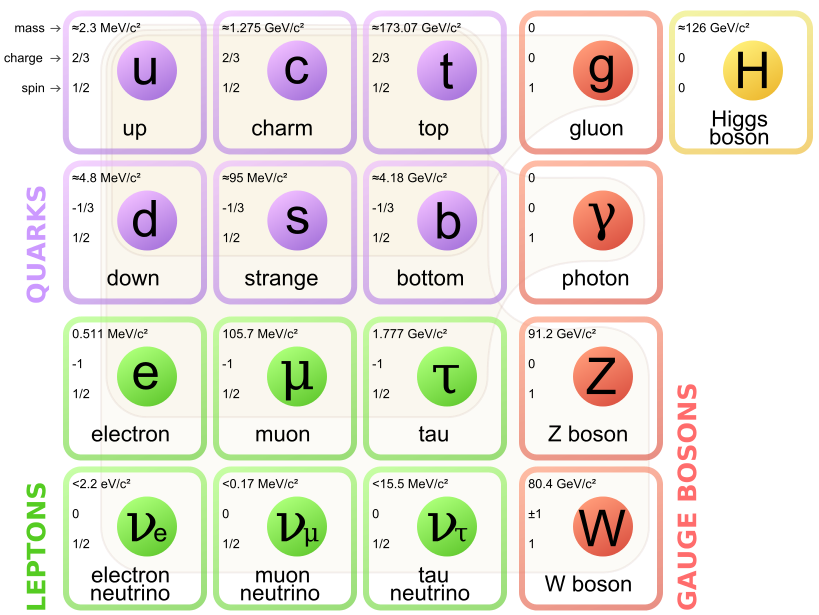
\includegraphics[width=0.7\textwidth]{images/standard-model.png}
\end{center}


\end{frame}


%------------------------------

\begin{frame}
\frametitle{Standard Model (SM)}

\begin{itemize}
\item SM predicts charge-parity (CP) conservation
\item SM predicts massless neutrinos
\item Both these are experimentally violated
\end{itemize}

\end{frame}


%------------------------------


\begin{frame}

\begin{center}
{\Huge Beyond the Standard Model}
\end{center}

\end{frame}

%------------------------------

\begin{frame}
\frametitle{Beyond the Standard Model - CP Violation}

\begin{itemize}
\item 
\end{itemize}

\end{frame}


%------------------------------


\begin{frame}
\frametitle{Beyond the Standard Model - Neutrino masses}

\begin{itemize}
\item Nobel Prize awarded in 2015 for ``\emph{the discovery of neutrino oscillations, which shows that neutrinos have mass}''
\item SM does not predict massive neutrinos
\item We need NP to explain neutrino mass generation
\item These NP mechanisms introduce LFV!
\end{itemize}


\end{frame}


%------------------------------



\begin{frame}

\begin{center}
{\Huge Motivation}
\end{center}

\end{frame}

%------------------------------


\begin{frame}
\frametitle{Motivation for the search}

\begin{itemize}
\item LFV probes GUT scale loops (high mass)
\item LFV is automatically introduced by neutrino mass generation mechanisms
\item Anomalies!
\end{itemize}

\end{frame}

%------------------------------


\begin{frame}

\begin{center}
{\Huge Anomalies}
\end{center}

\end{frame}

%------------------------------

\begin{frame}
\frametitle{Anomaly \#1: CMS Higgs excess ($h\to \tau\mu$)}

\begin{itemize}
\item CMS detected a $2.4\sigma$ excess in the branching fraction of $h\to\tau\mu$
\item \emph{Aristizabal Sierra, D.} and \emph{Vicente, A.} (2014) propose an explanation of the excess
\begin{itemize}
\item Type-III Two Higgs Doublet Model (2HDM)
\end{itemize}
\end{itemize}

\begin{center}
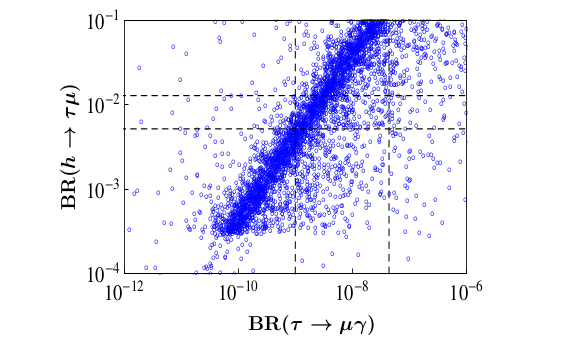
\includegraphics[width=0.7\textwidth]{images/h-tau-mu.png}
\end{center}


\end{frame}




%------------------------------

\begin{frame}
\frametitle{Anomaly \#2: Neutrino masses}

\begin{itemize}
\item in the SM with massive neutrinos, LFV is heavily suppressed by neutrino mass, proportional to GIM factor $\left(\frac{m_{\nu}}{M_W}\right)^2$
\end{itemize}

\begin{center}
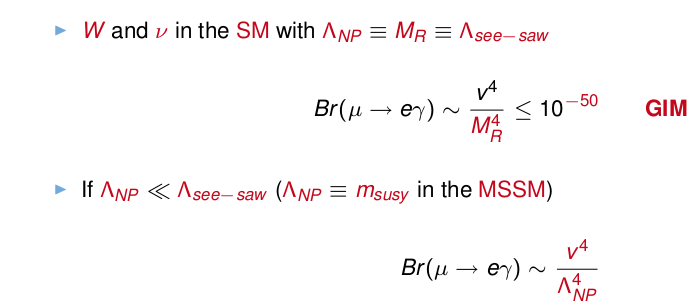
\includegraphics[width=\textwidth]{images/paradisi-mssm-br.png}
\end{center}


\end{frame}




%------------------------------


\begin{frame}

\begin{center}
{\Huge Lepton-Flavour Changing Processes}
\end{center}

\end{frame}

%------------------------------


\begin{frame}
\frametitle{Lepton-Flavour Changing Processes - Overview}

\begin{itemize}
\item LFV is introduced in NP by neutrino mass generation mechanisms
\item Some major models include ??? 
\item 
\end{itemize}

\end{frame}


%------------------------------


\begin{frame}

\begin{center}
{\Huge Other searches}
\end{center}

\end{frame}

%------------------------------

\begin{frame}
\frametitle{Other searches - overview}

\begin{itemize}
\item Belle (2007) 
\begin{itemize}
\item $\mathcal{B}(\tau^{-}\to\mu^{-}\gamma)<\SI{4.5d-8}{}$
\item $\mathcal{B}(\tau^{-}\to e^{-}\gamma)<\SI{12d-7}{}$
\end{itemize}
\item BaBar (2010)
\begin{itemize}
\item $\mathcal{B}(\tau^{-}\to\mu^{-}\gamma)<\SI{4.4d-8}{}$
\item $\mathcal{B}(\tau^{-}\to e^{-}\gamma)<\SI{3.3d-8}{}$
\end{itemize}
\end{itemize}

\end{frame}

%------------------------------
\begin{frame}
\frametitle{Other searches - overview}

\begin{columns}
\begin{column}{0.5\textwidth}
\begin{center}
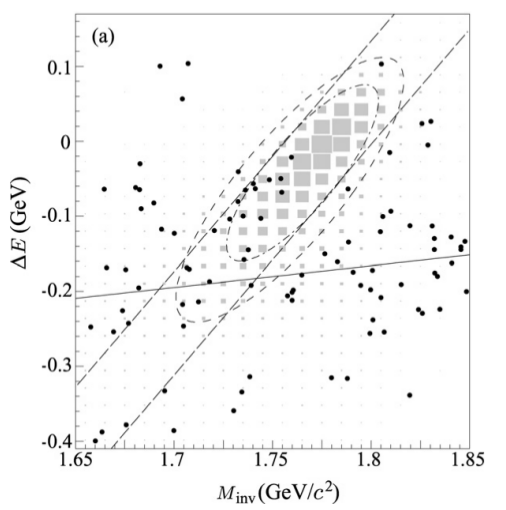
\includegraphics[width=\textwidth]{images/belle-mu-GSR.png}
\end{center}
\end{column}

\begin{column}{0.5\textwidth}
\begin{center}
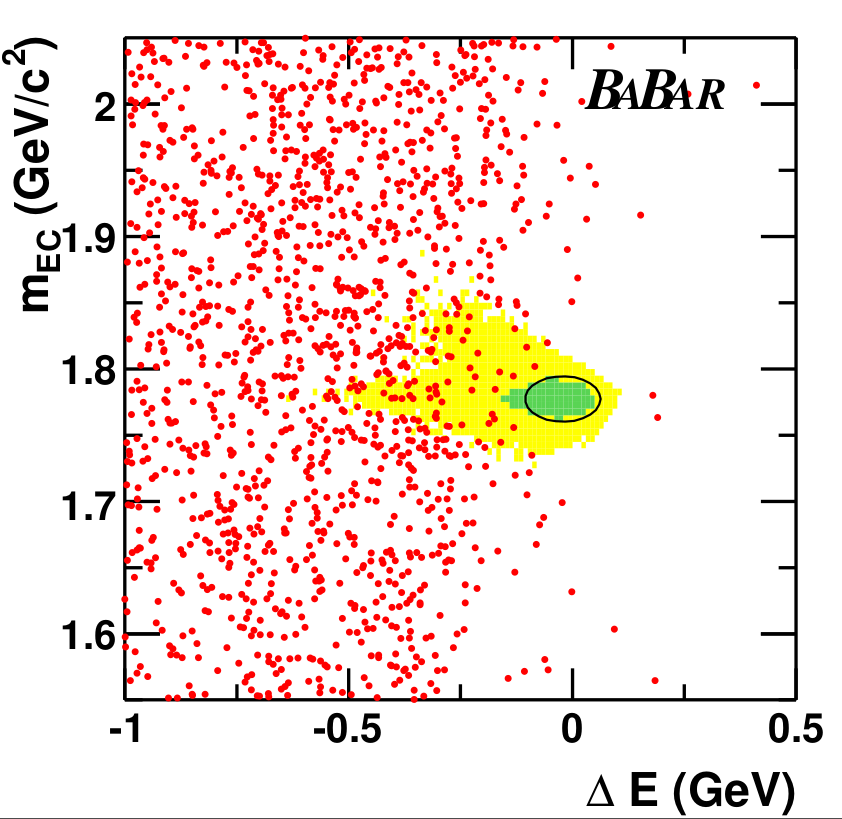
\includegraphics[width=\textwidth]{images/babar-mu-GSR.png}
\end{center}
\end{column}

\end{columns}
\end{frame}



%------------------------------
\begin{frame}
\frametitle{Other searches - overview}

\begin{center}
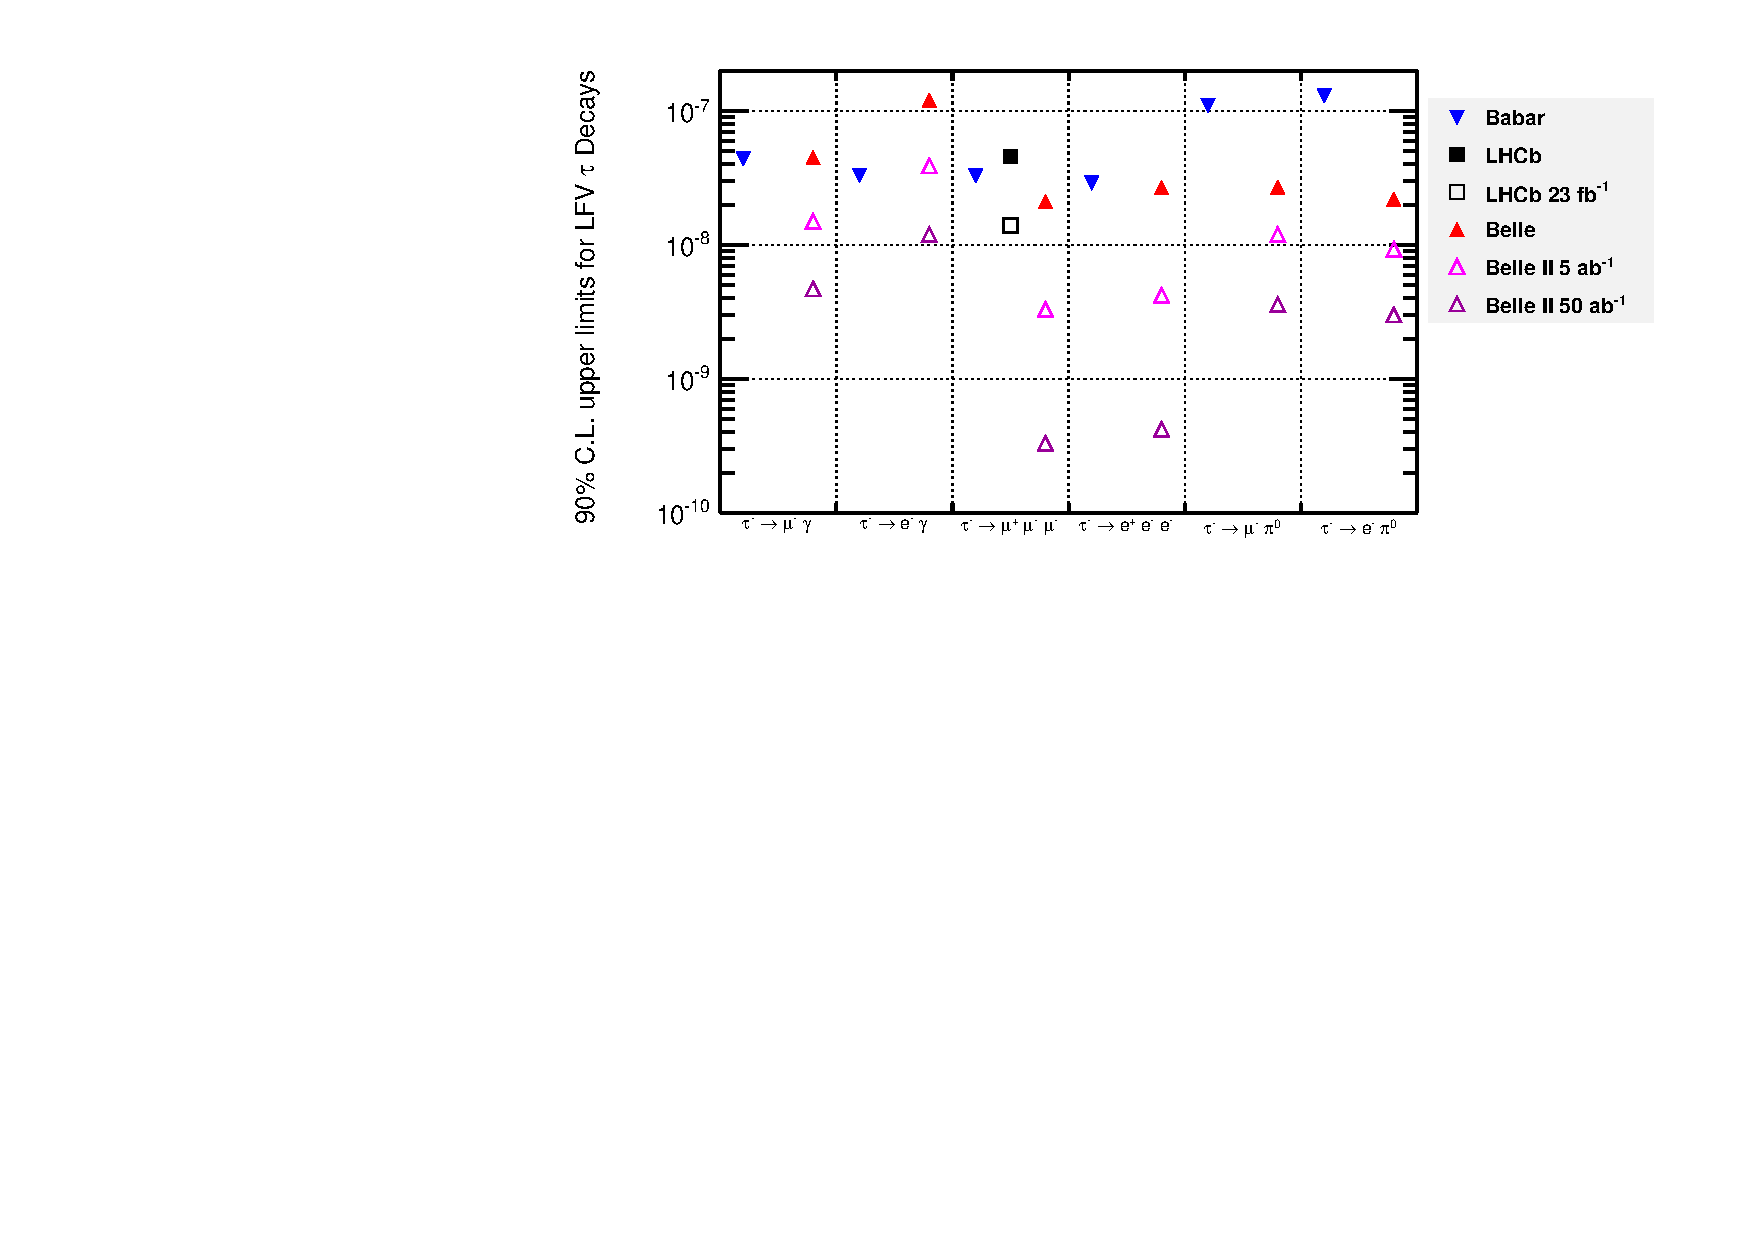
\includegraphics[width=\textwidth]{images/tauLFV.pdf}
\end{center}

\end{frame}


%------------------------------

\begin{frame}

\begin{center}
{\Huge Current progess}
\end{center}

\end{frame}

%------------------------------

\begin{frame}
\frametitle{Current progress - selection}


\begin{center}
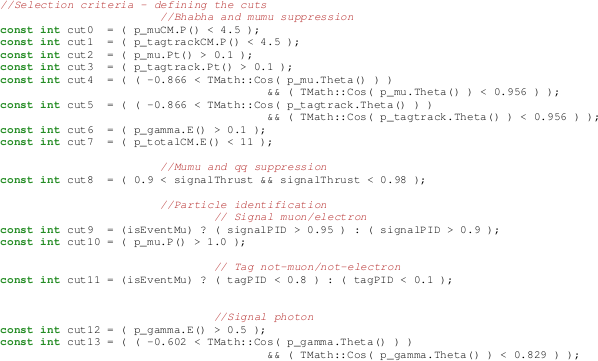
\includegraphics[width=0.8\textwidth]{images/selection-code1.png}
\end{center}

24 selection criteria, taken from previous Belle search (currently unoptimised).


\end{frame}

%------------------------------

\begin{frame}
\frametitle{Current progress - selection}


\begin{center}
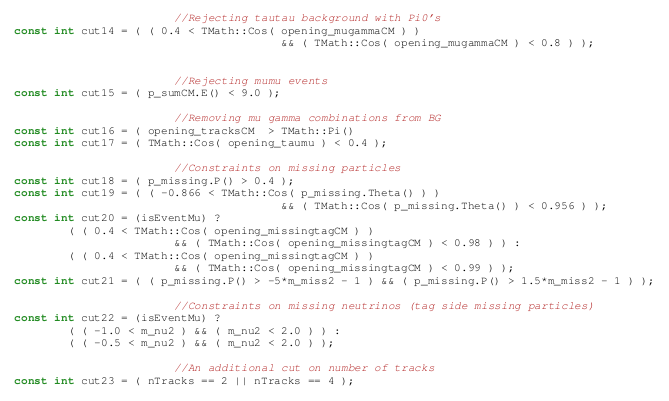
\includegraphics[width=0.8\textwidth]{images/selection-code2.png}
\end{center}

24 selection criteria, taken from previous Belle search (currently unoptimised).


\end{frame}

%------------------------------

\begin{frame}
\frametitle{Current progress - fitting region}

\begin{columns}
\begin{column}{0.5\textwidth}
\begin{center}
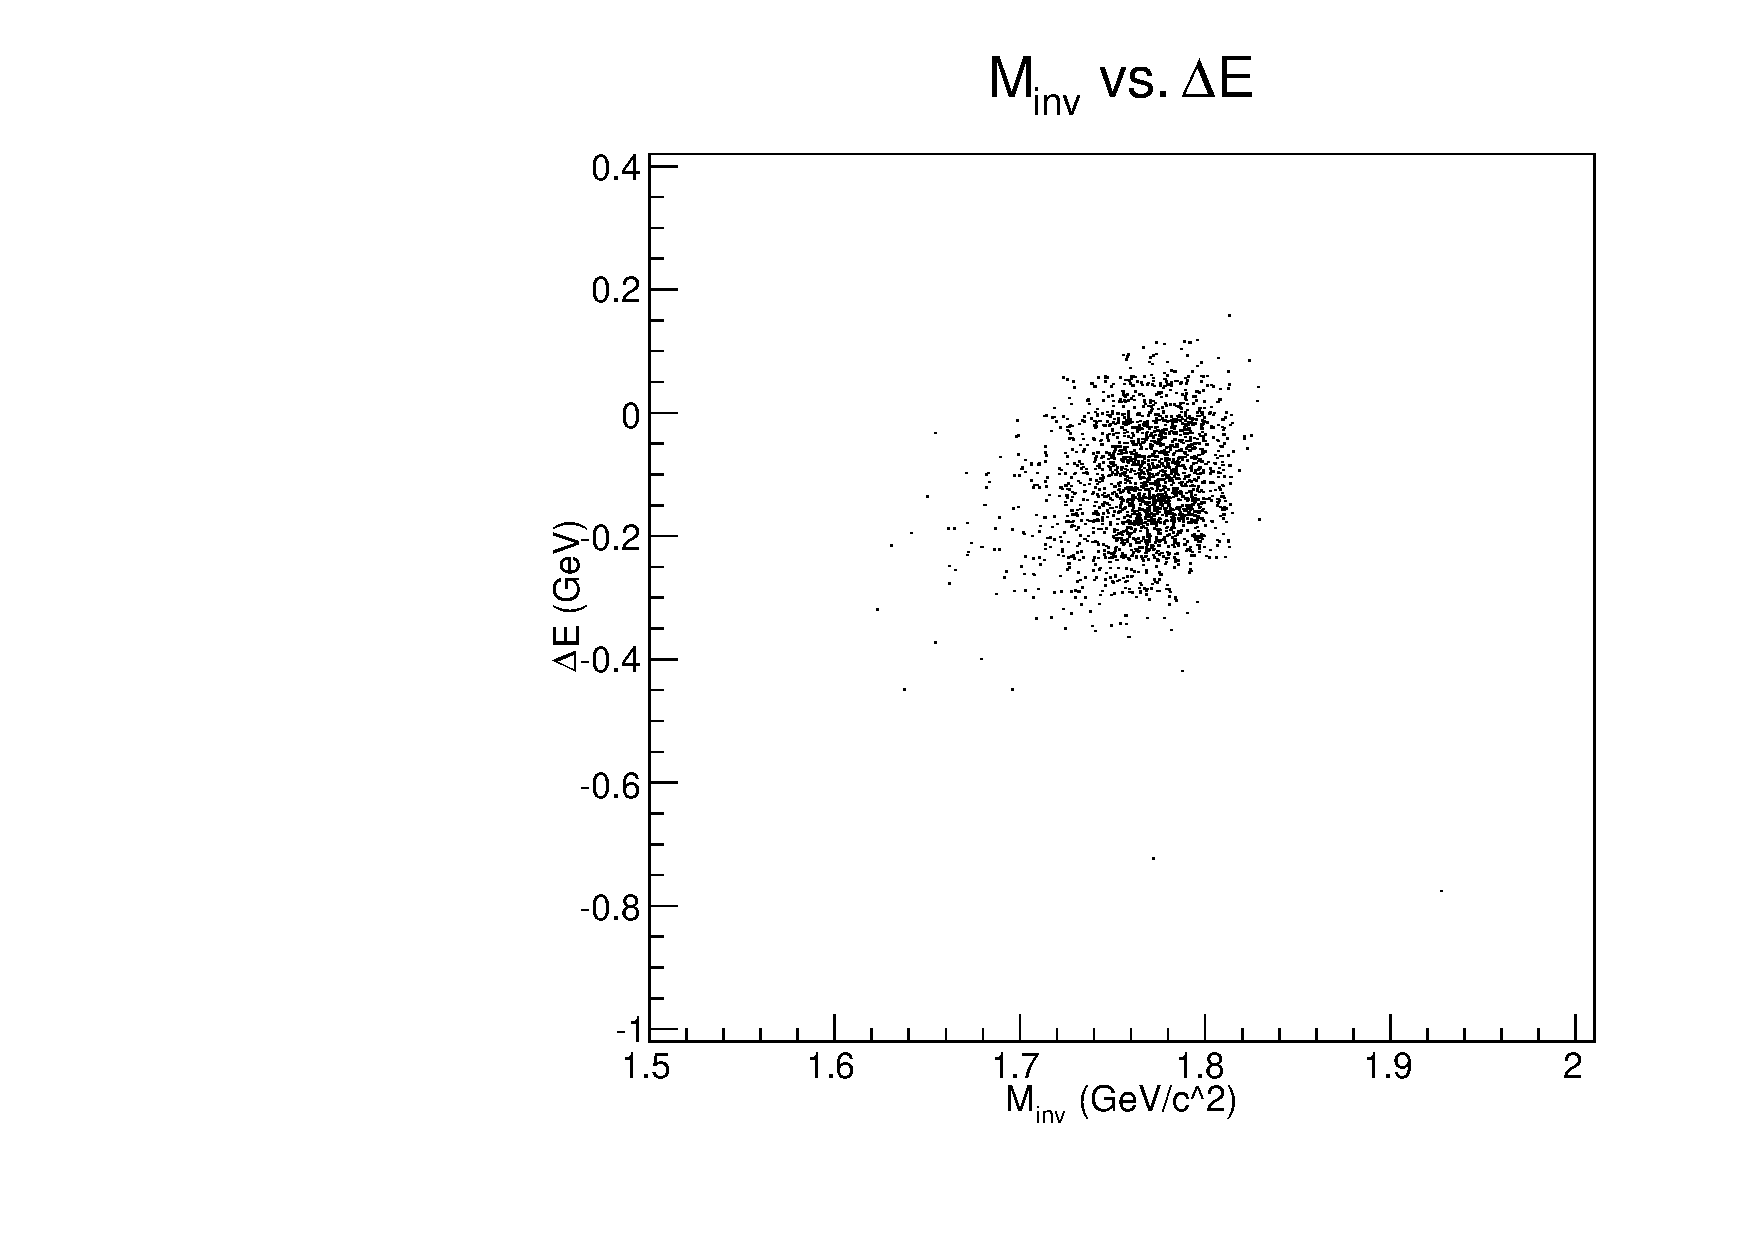
\includegraphics[width=\textwidth]{images/deltaE_vs_Minv_SIG.pdf}
\end{center}
\end{column}

\begin{column}{0.5\textwidth}
\begin{center}
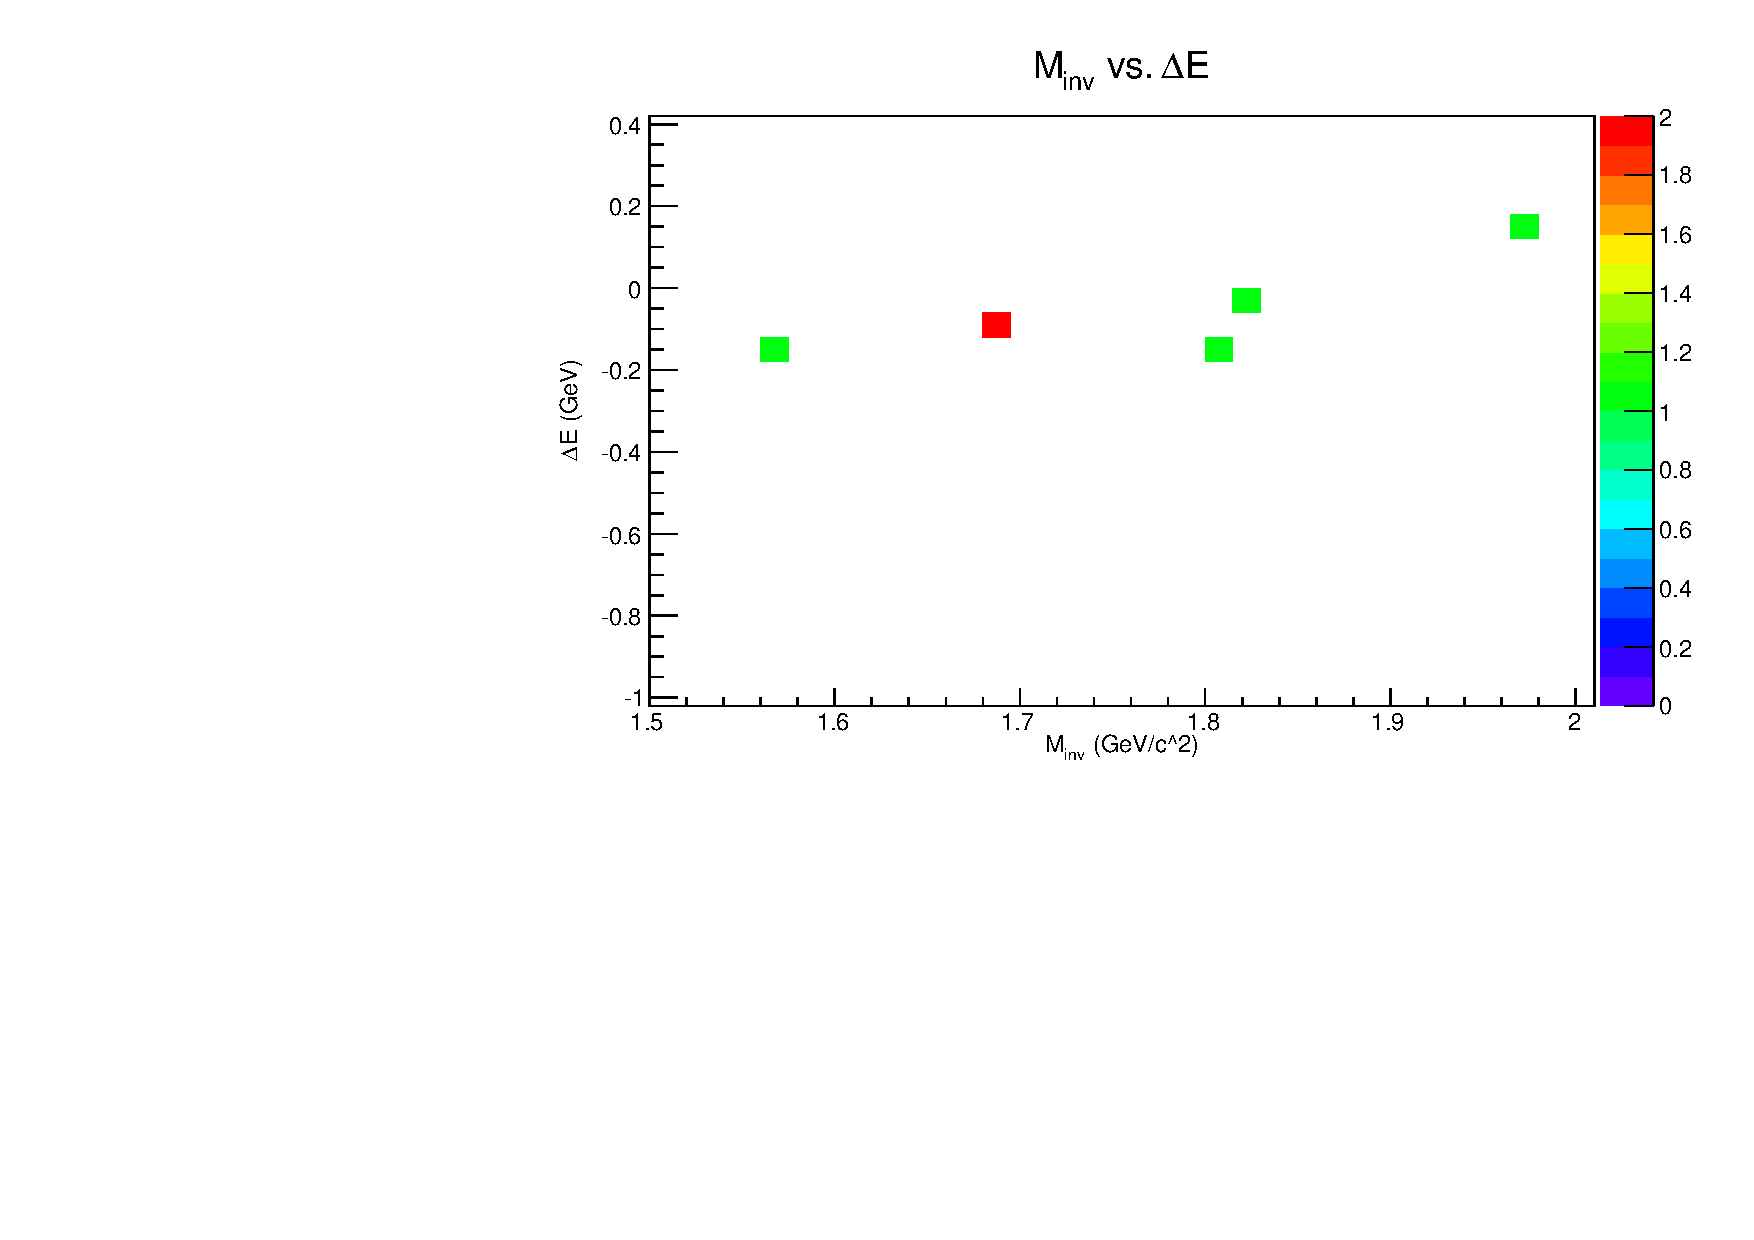
\includegraphics[width=\textwidth]{images/deltaE_vs_Minv_BG.pdf}
\end{center}
\end{column}

\end{columns}

We will select a region in our $M_{\text{inv}}$ vs. $\Delta E$ plots as our Grand Signal Region (where events will be selected from data.

\end{frame}

%------------------------------


\begin{frame}
\frametitle{Summary}

\begin{columns}
\begin{column}{0.7\textwidth}
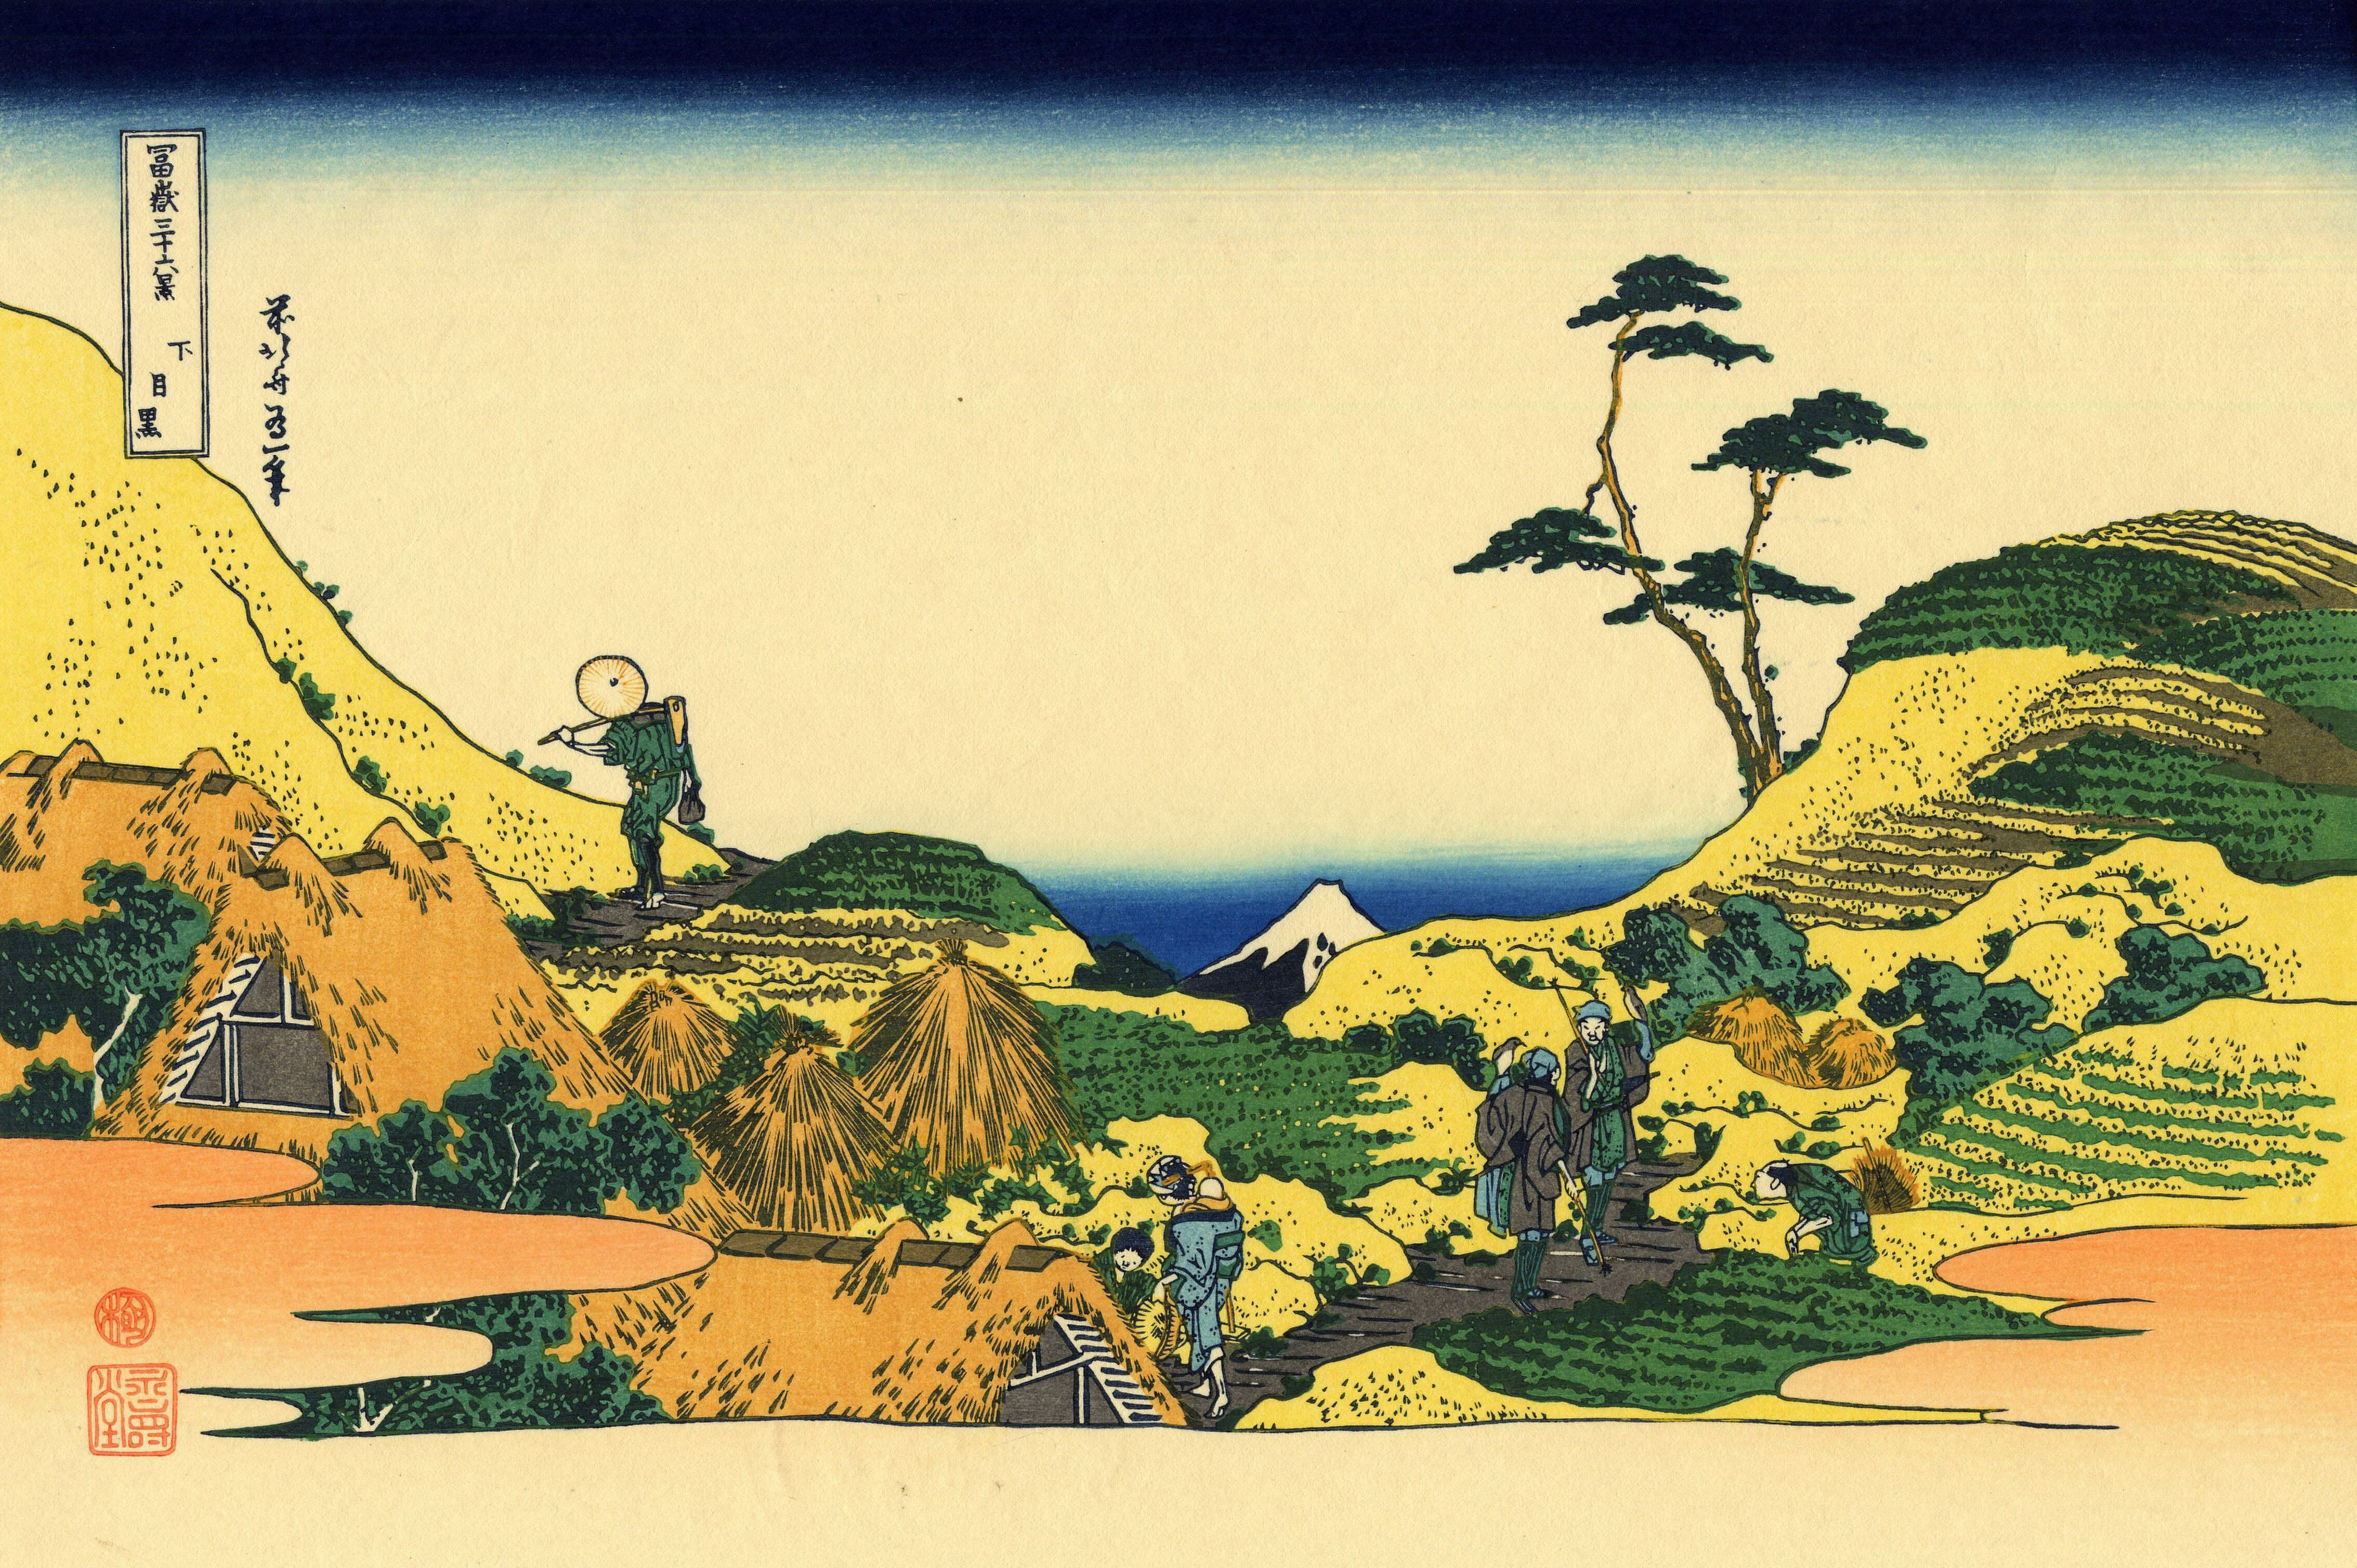
\includegraphics[width=\textwidth]{images/fuji15.jpg}
\end{column}
\begin{column}{0.3\textwidth}
Thanks.
\end{column}


\end{columns}

\end{frame}


%------------------------------


 
\end{document}






